\normalfalse \difficilefalse \tdifficiletrue
\correctionfalse

%\UPSTIidClasse{11} % 11 sup, 12 spé
%\newcommand{\UPSTIidClasse}{12}

\exer{Variateur à billes $\star\star\star\star\star\star$ \label{GEO:03:C2:06:19}}

\setcounter{question}{0}\UPSTIcompetence[2]{B2-13}\UPSTIcompetence[2]{C2-05}\marginnote{\xpComp{GEO}{03}}%\UPSTIcompetence[2]{C2-06}
\index{Compétence C2-05}
\index{Compétence C2-06}\index{Compétence GEO-03}
\index{Compétence B2-13}
\index{Variateur de Graham}
\ifcorrection
\else
\marginnote{\textbf{Pas de corrigé pour cet exercice.}}
\fi

\ifprof
\else

Soit le schéma suivant. 
\begin{marginfigure}
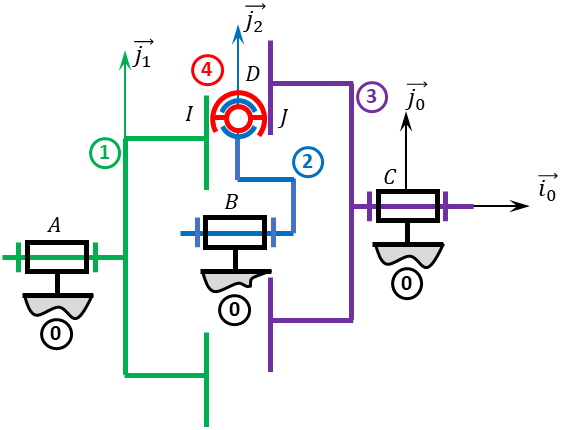
\includegraphics[width=\linewidth]{20_01}
\end{marginfigure}
\fi

\question{Tracer le graphe des liaisons.}
\ifprof
\else
\fi

\question{Déterminer la loi entrée -- sortie.}
\ifprof
\else
\fi


\ifprof
\else

\marginnote{Corrigé voir \ref{GEO:03:C2:06:19}.}

\fi